\chapter{Results of Experiments concerning \AspectOriented Modelling}
\label{chap:exp2_old_aspects_new_systems}
\label{chap:experimental_results}
\label{sec:optimisation_with_aspects_experimental_results}



The naive model of RPGLite and the \aspectoriented models of learning \&
confidence which are described in \cref{chap:experiment_setup} are designed to
answer the following research questions:

\begin{researchquestion}
  \begin{description}
\item[RQ2] \rqtwo{}
\item[RQ3] \rqthree{}
\item[RQ4] \rqfour{}
  \end{description}
\end{researchquestion}

% === Keeping this here for now --- think I might want to re-use it for talking
% === about the prior distribution model.
%To investigate these, the naive model of RPGLite play is augmented using the
%aspect-oriented models of learning outlined in
%\cref{sec:optimisation_with_aspects_aspectsdeveloped}. The datasets produced by
%executing both the unaltered naive model and the naive model with aspects
%applied are compared against the real-world dataset described in
%\cref{chap:rpglite}. Comparisons are made by quantifying the similarity of
%the character pair preferences found in each dataset as defined in
%\cref{measuring_charpair_similarity}. Whichever synthetic dataset is most
%similar to the empirically sourced one can be said to be the most realistic.
%This experiment has the null hypothesis that introducing aspects has no impact
%on model realism. If no change in model behaviour can be measured when learning
%models are applied, then it would be possible to \emph{represent} model changes
%as advice as demonstrated in
%\cref{sec:optimisation_with_aspects_aspectsdeveloped} but not possible to
%\emph{use} those changes in their aspect-oriented form.

To investigate each research question, relevant advice is woven into the naive
model, and datasets are generated of recorded simulated gameplay. To answer the
proposed research questions, these datasets are compared against the empirically
sourced datasets described in \cref{chap:rpglite}. Different experiments require
different comparisons and yield different contributions, but all make use of the
same foundations described in \cref{chap:experiment_setup}.

This chapter explores the results of the experiments which are enabled by the
previous chapter's foundations.
The first section describes how synthetic datasets are interpreted to yield
``optimal'' parameters when simulating a given player.
The second section explores an experiment answering the third research question,
concerning the use of advice to introduce new parameters and behaviours to a model.
The third section explores an experiment answering the fourth research question,
concerning the portability of advice as individual modules to new systems, or to
changed instances of the same system.
\inline{
  Add crefs to the sections mentioned here once they exist.
}



\section{Identifying Statistically Significant Results}
\label{exp_identiying_statistically_significant_results}

The process of generating datasets of simulated games of RPGLite outputs
datasets for each training fold which have a statistically significant
correlation to the real-world dataset produced by a player being simulated.
However, different folds may produce statistically significant results with
different parameters. For a model to represent a player's behaviour across all
folds, its parameters should be independent of the fold being compared against.
As a result, it is necessary to identify model parameters which produce
statistically significant behaviour across many training folds.

In scenarios where a player has many model parameters which provide
statistically significant results across a majority of folds, stronger results
should be preferred. However, a balance must be reached between the \tau{}
correlation coefficient and the p-value which denotes confidence in that
statistic: a low correlation statistic indicates little similarity between
datasets, and a high p-value indicates a high probability that any measured
correlation would occur when the null hypothesis is correct.\footnote{i.e. incidentally,
rather than as a result of a hypothesis being true.}

A set of model parameters yielding significant results for simulating a given
player are selected by identifying model parameters which produced results above
a threshold correlation coefficient and below a threshold p-value across $>50\%$
of folds. All sets of parameters meeting these thresholds are then used to
generate another dataset, the correlation of which is measured against the
empirical dataset of the simulated player. If the new dataset's correlation
meets the thresholds for correlation coefficient and p-value, it is considered
to accurately simulate the player. A result is therefore found. If no sets of
parameters meet these criteria, the thresholds are weakened, and the search
repeats, until the thresholds can no longer be weakened without compromising the
significance of the results they would produce.

Correlation coefficient thresholds are selected at $0.5$, $0.4$, $0.3$, and
$0.2$. P-value thresholds are $0.01$, $0.02$, $0.035$, and $0.05$. We prefer a
weaker pvalue to a weaker correlation coefficient, as reliable weak correlation
is preferable to dubious strong correlation. For this reason, correlation
coefficient thresholds are relaxed only when all p-value thresholds have been
tested. The algorithm implementing this search is given in
\cref{search_for_correlation_coefficients} for reference.

The result of this search is that --- if they exist --- the model parameters are
returned which achieve optimally statistically significant results when
simulating a given player.



\section{RQ2: Altering Model Behaviour using \AspectOrientation}
\label{rq2_results}

\subsection{Experimental Design}

To demonstrate the viability of altering a model by using aspects to describe a
change in behaviour, the advice applying the already-known character pair
distribution to character pair selection is applied. This forms the first of
three experiments in this chapter, addressing the research question:

\begin{researchquestion}
\rqtwo{}
\end{researchquestion}

The research question yields a null hypothesis: \emph{models of systems cannot
be altered using advice to reflect their subjects more accurately}. If this were
the case, there would be no discernable difference between the real world data's
correlation against data from the naive model and data from a model with advice
woven. Simulated players in the naive model select character pairs randomly,
meaning that --- if patterns such as personal preference exist in the real-world
data, or the data is not randomly distributed --- we would not expect much
correlation between the two. If weaving advice produces datasets which do
correlate with the real-world data, then the advice would have affected the
model to more accurately reflect the player being simulated. We would therefore
discount the null hypothesis, and answer the research question affirmatively. If
no correlation could be produced as a result of weaving aspects, then the null
hypothesis would have been demonstrated instead, answering the research question
negatively.

\begin{figure}[h]
  \centering
  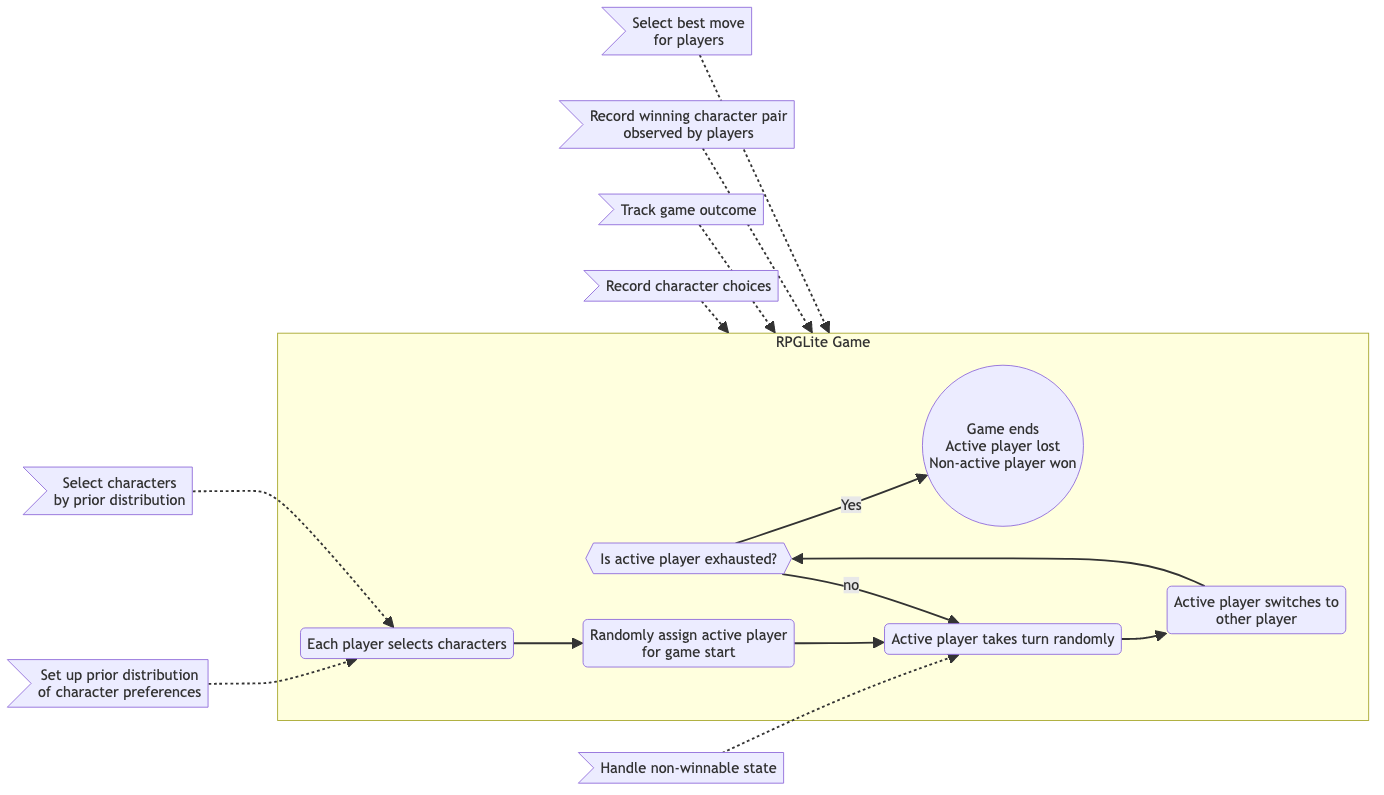
\includegraphics[width=\columnwidth]{70_generality_of_aspects/diagrams/exp2_prior_distribution_model.png}
  \caption{Advice woven into the naive model to adopt the distribution used to select character pairs from real-world data.}
  \label{fig:exp2_prior_distribution_model}
\end{figure}

\Cref{fig:exp2_prior_distribution_model} illustrates the advice woven into the
naive model to alter player behaviour to select character pairs with the same
distribution as the real-world data exhibits. As this advice causes simulated
players to select character pairs with the same distribution as real-world
players, the datasets generated using them ought to correlate strongly with the
real-world data: rather than being random, the distribution is expected to be
the same. This therefore tests our hypothesis that advice can be used to alter
model behaviour to be more accurate.
\footnote{
  Later experiments will investigate the addition of specific behaviours, rather
  than reproducing properties of an already-present dataset.
}


\subsection{Results}

The actual results we found.



\begin{figure}[h]
  \centering
  
  \begin{minipage}{.45\textwidth}
    \centering
    \begin{tabular}{r|c|c}
      \emph{Username} & \emph{p-value} & \emph{\tau{} statistic} \\\hline\hline
      apropos0 & 0.025 & 0.338 \\
      basta & 0.049 & 0.193 \\
    \end{tabular}
    \caption{Correlation of real-world character pair selection and those generated by an unmodified naive model}
    \label{prior_distribution_results_table_comparison_to_real_world_datasets}
  \end{minipage}\hfill
  \begin{minipage}{.45\textwidth}
    \centering
    \begin{tabular}{r|c|c}
      \emph{Username} & \emph{p-value} & \emph{\tau{} statistic} \\\hline\hline
      apropos0 & 0.025 & 0.338 \\
      basta & 0.049 & 0.193 \\
    \end{tabular}
    \caption{Correlation of real-world datasets of character pair selection and those generated by the naive model with advice woven to bias the characters chosen}
    \label{prior_distribution_results_table_comparison_to_real_world_datasets}
  \end{minipage}

\end{figure}




\subsection{Answering the Second Research Question}

A discussion of the second RQ, delivering a concrete answer using the results.
This doesn't have to be overly long.



\section{RQ3: Adding Model Behaviours \& Parameters using \AspectOrientation}
\label{rq3_results}

Applying our model of learning to add new behaviours to the model, and
parameters which control those behaviours.

\subsection{Experimental Design}

Details of this experiment specifically: what are we looking for? How will we
look for it? What is our hypothesis and null hypothesis, and how will this be
tested?

\subsection{Results}

Results drawn from running the RPGLite naive model with our model of learning
woven in.


\begin{figure}[h]
  \centering
  
  \begin{minipage}{.7\textwidth}
    \centering
    \begin{tabular}{r|c|c}
      \emph{Username} & \emph{p-value} & \emph{\tau{} statistic} \\\hline\hline
      apropos0 & 0.025 & 0.338 \\
      basta & 0.049 & 0.193 \\
    \end{tabular}
    \caption{Correlation of real-world datasets of character pair selection and those generated by applying the \aspectoriented model of learning}
    \label{learning_model_results_table_comparison_to_real_world_datasets}
  \end{minipage}
  
\end{figure}




\subsection{Answering the Third Research Question}

A discussion of the third RQ, delivering a concrete answer using the results.
This doesn't have to be overly long.





\section{RQ4: Applying Aspects to New Models}
\label{rq4_results}

The outcome of applying each of the earlier models to S2, keeping the same
parameters as were found to be most statistically significant in RQ3.

\subsection{Experimental Design}

Details of this experiment specifically: what are we looking for? How will we
look for it? What is our hypothesis and null hypothesis, and how will this be
tested?

\subsection{Results}

Results drawn from applying the parameterised models of play from both the prior
distribution model and the model of learning, ran on S2 instead of S1. Do we
still get decent correlation? Are the results useful?



\begin{figure}[h]
  \centering
  
  \begin{minipage}{.45\textwidth}
  \centering
  \begin{tabular}{r|c|c}
    \emph{Username} & \emph{p-value} & \emph{\tau{} statistic} \\\hline\hline
    apropos0 & 0.025 & 0.338 \\
    basta & 0.049 & 0.193 \\
  \end{tabular}
  \caption{Correlation for simulation using simple character pair distribution model on RPGLite Season 2}
  \label{prior_distribution_model_results_s2}
  \end{minipage}\hfill
  \begin{minipage}{.45\textwidth}
  \centering
  \begin{tabular}{r|c|c}
    \emph{Username} & \emph{p-value} & \emph{\tau{} statistic} \\\hline\hline
    apropos0 & 0.025 & 0.338 \\
    basta & 0.049 & 0.193 \\
  \end{tabular}
  \caption{Correlation for simulation using \aspectoriented model of learning on RPGLite Season 2 (with parameters selected in \cref{rq3_results})}
  \label{learning_model_results_s2}
  \end{minipage}
  
  % \caption{Correlation of real-world datasets of character pair selection and those generated by the tables' respective models, used to simulate to RPGLite Season 2 gameplay.}

\end{figure}





\subsection{Answering the Fourth Research Question}

A discussion of the fourth RQ, delivering a concrete answer using the results.

There are two perspectives here: first, simple aspects which are more oblivious
to the system they're applied to are more portable. The parameters of the model
of learning need to be fitted, and it turns out they're being fitted to both the
player \emph{and} the season: changing the season decimates the accuracy of the
model, so clearly the parameters aren't independent of the system they're being
fitted against. However, the prior distribution model is entirely independent of
season, and it works a treat. The result is that the advice being ported
matters, and while some advice \emph{can} be moved to new systems in a way that
makes sense, other advice will be invalidated by the change. A researcher
applying aspects to new systems therefore needs to demonstrate that they're
valid on the new system --- it could be a worthwhile endeavour to port advice
(instead of writing it from scratch) but there's still work involved.





\section{Discussion}

A brief overview of what was achieved in the three experiments discussed in this
chapter. Lots of contributions!
\revnote{
  I haven't added a section on the hyperbolic decay model, \emph{but} I have two
  implementations: one using ``within''-style weaving, and the other using
  traditional join points. It'd be interesting to compare them. Perhaps this
  actually belongs in e.g. the \pdsf rewrite chapter.
}




%\subsection{Identifying Statistically Significant Results in Datasets}
%
%\inline{
%  A discussion of how datasets are evaluated. We produce \emph{many} datasets
%  which have annealed to the highest stat and P val we could find, but they're
%  split across many folds. How do we determine whether a set of parameters works
%  ``enough''? We find the highest correlation val and lowest pval which work
%  across a majority of folds, then test against the complete dataset to be
%  absolutely certain that correlation doesn't drop. This gives us the best
%  parameters for a player: the parameters were reliably annealed to across many
%  folds to give statistically significant correlation, retained their
%  correlation against a testing set, and further retained their correlation
%  against the entire dataset.
%}
%
%\inline{
%  Is there a pattern in players getting reliable correlation and having played
%  many games? Maybe we just don't have enough games to do this for most players.
%  Check this; could be worth a note toward the end, in a discussion or similar.
%}
%
%\inline{
%  This is an explanation of the analysis script, not the process f annealing; we
%  should already have that in the experimental design section (currently 6.5, at
%  time of writing).
%}
%
%
%
%
%
%\subsection{Selecting Character Pairs from a Known Distribution}
%
%The second research question presented in \cref{subsec:rqs} is:
%
%\begin{researchquestion}
%  Can a model be made more realistic by applying aspect-oriented improvements?
%\end{researchquestion}
%
%This question can be answered directly by weaving advice which modifies player
%behaviour so that character pairs are selected from a distribution calculated
%from existing player data. If the dataset produced with this advice woven
%correlates with the pre-calculated distribution of character pair preferences,
%then the simulated behaviour must have been affected by the aspects in the
%manner the advice modelled, and so made the model more realistic. If the dataset
%correlates with that produced by the naive model, it must have had no effect.
%And, if it correlates with neither, then the weaving of advice modelling a
%specific character pair selection did impact player behaviour, but did not
%produce expected results.\footnote{In this scenario, there would likely be an
%error in implementation as the aspects demonstrably made a difference to
%behaviour, but not what was intended. Rather than confirming the hypothesis that
%advice can be used to augment models of behaviour or the null hypothesis that
%weaving such advice has no effect, it would indicate a flawed experiment.}
%
%Datasets representing every real-world player who completed more than 100 games
%in RPGLite's first season were generated with the advice described in
%\cref{sec:optimisation_with_aspects_aspectsdeveloped} woven. There were 21 such
%players. The \tau correlation statistic (and corresponding p-values) of these
%datasets compared to their players'
%real-world datasets and the naive model's dataset is presented in
%\cref{fig:known_distribution_results_s1}.
%
%\begin{figure}[h]
%\begin{center}
%  \begin{tabular}{c|c|c}
%    \emph{Simulated Player} & \emph{P-Value} & \emph{Correlation Statistic} \\ \hline\hline
%    Data1 & data2 & data3 \\
%    Data1 & data2 & data3 \\
%  \end{tabular}
%  \caption{Correlation statistics generated by weaving aspects into the naive
%    model which select character pairs with the same distribution as a specific
%    real-world player}
%  \label{fig:known_distribution_results_s1}
%\end{center}
%\end{figure}
%
%
%
%\inline{TODO: add notes explaining what an acceptable pval and correlation stat
%  are. This will be useful to refer back to in the next subsection, where not
%  all players are simulated by each model.}
%
%
%\inline{Explain the results \& relate them to the final RQ.}
%
%
%
%\subsection{Selecting Character Pairs using Confidence-Based Learning}
%
%\inline{I suspect I'll move this to the discussion of the next experiment, so
%  that the aspects using the known distribution are presented as an
%  investigation of the first research question, and the aspects using the
%  confidence-based model of learning are presented as an investigation of the
%  second.}
%
%Selecting character pairs based on a known distribution demonstrates that advice
%can alter the behaviour of actors in a model, improving the model's accuracy.
%
%\inline{I'm increasingly realising that the aspect drawing from a known
%  distribution is both more accurate and more portable than our models of
%  learning: we can apply it to S2 and just draw from season-specific data to get
%  the correct results. It's actually way better than our models of learning.
%  However, the models of learning let us investigate specific players'
%  behaviour, so they let us use the naive model to investigate the bahviour of
%  real-world players, which is still quite valuable, but might want a different
%  approach to the write-up. I'm pretty lost with this chapter --- need Tim's
%  input, I think.}
%
%
%
%%This is a relatively short chapter; a lot of the building blocks for it exist in
%%the previous chapter, so there's less ground to cover. If it ends up quite
%%lop-sided, I'd chop the earlier chapter in two rather than artificially making
%%this chapter beefier; I think it'd flow better.
%
%This needs rewriting (and re-titling!) --- it's now a chapter on the results for
%all the experiments, including the three RQs:
%
%\begin{itemize}
%  \item \rqtwo{}
%  \item \rqthree{}
%  \item \rqfour{}
%\end{itemize}
%
%\section{(Reword) Experimental motivations / motivation of research question}
%This section should describe why it's interesting to move an aspect trained on
%some actors' behaviours to a new system, and discuss what investigating this can
%teach us that we \emph{don't} already know from the previous experimental
%chapter. We've got aspects which represent behavioural variance. If the system
%changes, can we expect that these aspects still apply to the new system? Is the
%representation of behavioural variance in this model separable from the system
%the behaviour occurs within?
%
%\subsection{Coupling of Model and Behaviour}
%Explaining the issues of behaviour coupled to models. Highly related to some of
%the reviewed literature --- I forget exactly what --- which discussed whether
%aspects which were designed to be applied to one system could feasibly be
%transferred to other systems, or whether they're inherently aware of the system
%they're originally designed for. The core concept is that to be making changes
%to some underlying codebase, you probably have to know what that codebase is, in
%most cases at least.
%
%\subsection{(Reword) Gaps/opportunities left by previous experiment}
%In the previous experiment we demonstrated that behavioural variance can be
%plausibly realistic. Are those variations separable from their underlying model,
%or --- when trained i.e. made realistic --- do they suffer from the coupling
%discussed in the previous subsection?
%
%\subsection{Research Question}
%Whatever the specific research question's wording for this was. Something about
%decoupling realistic aspects from a given model maybe? It should be in an
%earlier chapter somewhere.
%
%\section{Experimental Design}
%We took old player data and trained aspects on them, and in the previous
%experiment we found they were statistically significantly accurate. We ran a
%second season of RPGLite with slightly different parameters on player data. We
%modelled how players learned and variations on their learning patterns, so in
%theory, we should be able to apply the new learning patterns to the other system
%too. Do we have to re-train the aspects? How portable are they? This section
%lays out the design of this experiment.
%
%
%\subsection{Changes to RPGLite}
%What changes did we make to our system?
%
%
%\subsection{Applying Behavioural Variations to New System}
%Layout of new experiment, how it'll work, what's measured, why it should answer
%the RQ.
%
%
%\section{Applying Aspects from a Control System to a New System}
%Our implementation \& results from the experiment described above. Discusses how
%the above experiment was realised, lays out the results we found, and relates
%those results to the research question we started with.
%
%\subsection{Implementation}
%Implementation of the experiment
%
%\subsection{Results}
%Presentation of the results of the experiment, analysis, some discussion (more
%in next section too)
%
%\section{Discussion}
%Some notes discussing the outcome of this research question (that trained
%aspects representing behavioural variance aren't separable from the system
%they're trained around)

